\chapter{Towards better understanding of relational latent representations}\label{ch:embeddinganalysis}


This chapter focuses on analysing the properties of relational latent representations.
It focuses on explaining the effectiveness of such representation transformations and establishing the relative advantages of \gls{kge}s compared with the methods within the \gls{srl} methods and vice versa.
This chapter is based on the following publications:

\begin{quote}
	\bibentry{Dumancic2017b}
\end{quote}


\begin{quote}
	\bibentry{Dumancic2018}
\end{quote}

\begin{quote}
	\bibentry{AnalysisSubmitted}
\end{quote}

\section{Introduction}





A common criticism of  (relational) representation learning methods concerns their black-box nature.
Latent features are created through layers of non-linear transformations which are often incomprehensible as the neural architectures implementing the transformation can easily have up to several billions of parameters.
It is also difficult to know which kind of knowledge latent features capture nor \textit{why} that particular knowledge is useful for the prediction.
As both entities and relations are mapped to the points in the Euclidean space, \gls{kge}s thus approximate the original data.
We currently lack any measure to assess the quality of such approximation, nor do we know how to associate semantics to relations and entities in the Euclidean space.



This chapter introduces two sets of experiments that offer more insight into the effectiveness of relational latent representations.
The first set of experiments investigates why representations created by \gls{curled} are effective and identify two properties that correlated well with the increase in the performance of the \gls{srl} methods.
The second set of experiments compares several state of the art \gls{kge} and \gls{ilp} methods on several benchmark datasets, including both relational classification and knowledge base completion.
The experiments are designed to gain insights into relative strengths and weaknesses of the respective methods.
The experiments reveal several indicators that might help in choosing one method over another one for a specific  relational dataset.






%In [18], a contrast is presented between theories that predict everything, but
%explain nothing; and those that explain everything, but predict nothing. Both
%are seen as having limited value in the scientific enterprise, which requires models
%with both predictive and explanatory power




\section{Why are CUR$^2$LED representations effective?}


Latent features produced by \gls{curled} have proven useful in reducing the complexity of models and improving their performance.
However, no explanation was offered why that is the case.
In this section, we look into the properties of these latent representations and offer a partial explanation for their usefulness.
To answer this question we introduce the following properties: label entropy, sparsity and redundancy.



Label entropy and sparsity serve as a proxy to a quantification of learning difficulty -- i.e., how difficult is it to learn a definition of the target concept.
Considering a particular predicate, label entropy reflects a \textit{purity} of its true groundings with respect to the provided labels.
Intuitively, if true groundings of predicates tend to predominantly focus on one particular label, we expect model learning to be easier.


Sparse representations, one of the cornerstones of deep learning \cite{Bengio2013RLR}, refer to a notion in which concepts are explained based on local (instead of global) properties of instance space.
Even though many properties might exist for a particular problem, sparse representations describe instances using only a small subset of those properties.
Intuitively, a concept spread across a small number of local regions is expected to be easier to capture than a concept spread globally over an entire instance space.



Quantifying sparsity in relational data is a challenging task which can be approached from multiple directions -- either by analysing the number of true groundings or interaction between entities, for instance.
We adopt a simple definition: the number of true groundings of a predicate.


Label entropy and sparsity jointly describe a compelling property of data representation --  instances space is divided into many local regions that match labels well  and consequently make learning substantially easier.



\textbf{Redundancy.}
A downside of CUR$^2$LED is the high number of  created features.
Despite their proven usefulness, a high number of latent features enlarges the search space of a relational model and increases the difficulty of learning.
As similarity interpretations are provided by the user, it is possible that almost identical clusterings are obtained with different similarity interpretations.
Thus, if many of the features are redundant, removing them simplifies learning.

We measure the redundancy with the \textit{adjusted Rand index} (ARI) \cite{Rand71,MoreyARI}, a standard measure for overlap between clusterings, and study its impact on the performance.
To evaluate the influence of redundant features, we modify CUR$^2$LED by adding an additional \textit{overlap parameter} $\alpha$.
Every time a new clustering is obtained, we check its overlap with the previously discovered clusterings using the ARI.
If the calculated value is bigger than $\alpha$, the clustering is rejected.



\subsection{Experiments and results}

We devise the experiments to answer the following questions:
\begin{itemize}
    \item[\textbf{(Q1)}] \textit{Do latent features that result in models of lower complexity and/or improved performance exhibit a lower label entropy compared to the original data representation?}
    \item[\textbf{(Q2)}] \textit{Are latent representation that improve the performance of a model sparser than the original data representations?}
    \item[\textbf{(Q3)}] \textit{To which extent are latent features redundant?}
\end{itemize}

\subsubsection{Datasets and setup}

The results  obtained in \cite{Dumancic2017} can be divided in three categories.
The first category contains the IMDB and UWCSE datasets; these datasets present easy relational learning tasks in which the original data representation is sufficient for almost perfect performance.
The main benefit of latent representations for these tasks was the reduction of model complexity.
The second category includes the TerroristAttack dataset, in which the main benefit of latent representation was the reduction of complexity, but not the performance.
The third category involves the Hepatitis, Mutagenesis and WebKB datasets.
These tasks benefited from latent representations in both performance and reduced model complexity.
That is especially true for the Hepatitis and WebKB datasets on which the performance was improved by a large margin.


We take a representative task from each of the categories.
Precisely, we use IMDB, UWCSE, Hepatitis and TerroristAttack datasets in our experiments.
Both IMDB and UWCSE datasets were included as they are easy to understand without the domain knowledge, and thus useful for analysing the interpretability of relational latent features.
As for the parameters of latent representation, we take the best parameters on individual datasets selected by the model selection procedure in \cite{Dumancic2017}.
When analysing the interpretability, we set $\theta$ to $0.3$.

When evaluating the redundancy, we create latent representations by setting the $\alpha$ to the following values: $\{0.9, 0.8, 0.7, 0.6, 0.5\}$.
We then learn a relational decision tree \gls{tilde} on the obtained representation and compare accuracies, the number of created features and the number of facts.


When analysing the entropy and sparsity of representations, predicates indicating labels (such as \texttt{Professor} or \texttt{Student}) and entity definitions (such as \texttt{Person} or \texttt{Course}) are not considered in the analysis.


\subsubsection{Results}


\begin{figure}[t]
	\centering
	\medskip
    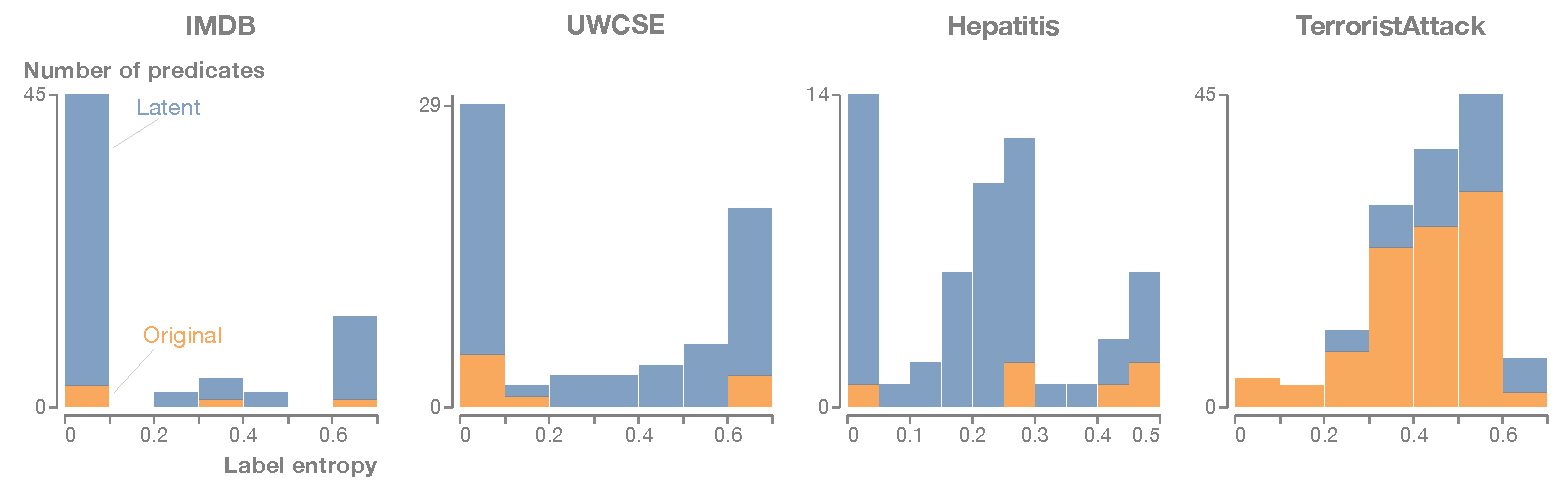
\includegraphics[width=1\textwidth]{entropy}
    \caption[Label entropy of latent representation created by \gls{curled}]{Latent representations for IMDB, UWCSE and Hepatitis datasets contain substantially larger number of predicates (and the corresponding facts) with low label entropy, compared to the original representation of data. On the TerroristAttack dataset, for which the latent representation has not been useful, that is not the case - both original and latent representation demonstrate similar trends in label entropy of the predicates and the corresponding facts.}
    \label{fig:Entropy}
\end{figure}


\textbf{Label entropy.}
Figure~\ref{fig:Entropy} summarises the label entropy for each dataset.
In all cases where representation learning proved helpful (i.e., IMDB, UWCSE, Hepatitis), latent representations have a substantially larger number of predicates with low label entropy compared to the original data representation.
The latent representation for the TerroristAttack datasets, however, shows a different behaviour in which latent features with high entropy dominate the representation.
These results agree with the expectation that a high number of low entropy features makes learning easier.
However, not all latent features have low label entropy.
This is expected, as the labels are not considered during learning of latent features.
It also does not pose a problem -- these latent features are less consistent with the one particular task, but it might well be the case that those features are useful for a different task.




\begin{figure}
	\centering
	\medskip
    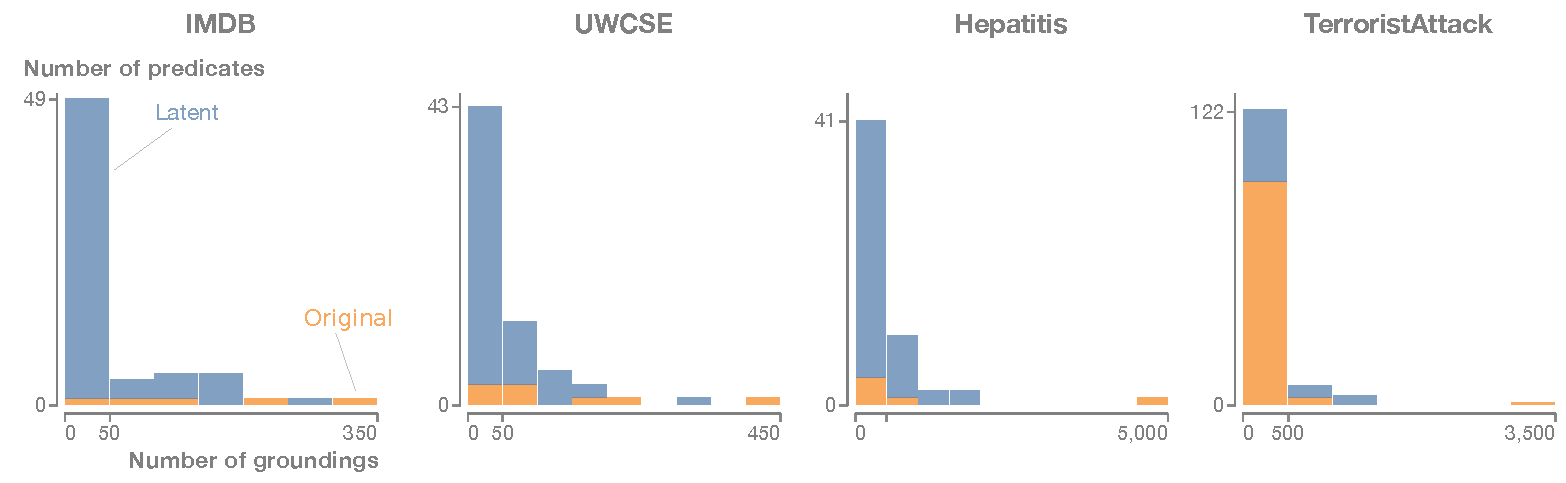
\includegraphics[width=1\textwidth]{sparsity}
    \caption[Sparsity of latent representation created by \gls{curled}]{Latent representation tends to be sparser than the original representation on the datasets where it is beneficial (IMDB, UWCSE and Hepatitis). On the TerroristAttack dataset, where the latent representation is not beneficial, both original and latent representation follow the same trend. }
    \label{fig:Sparsity}
\end{figure}


\textbf{Sparsity.}
Figure~\ref{fig:Sparsity} summarises the sparsity results in terms of the number of true instantiations of predicates.
The distribution of the number of true groundings in the latent representations (where latent features are beneficial) is heavily skewed towards a small number of groundings, in contrast with the original representation.
That is especially the case with the Hepatitis dataset, which profits the most from the latent features.
The exception to this behaviour is again the TerroristAttack dataset in which the original representation already is very sparse.
These results indicates that latent features indeed describe smaller groups of instances and their local properties, instead of global properties of all instances.





\begin{figure}
	\centering
	\medskip
    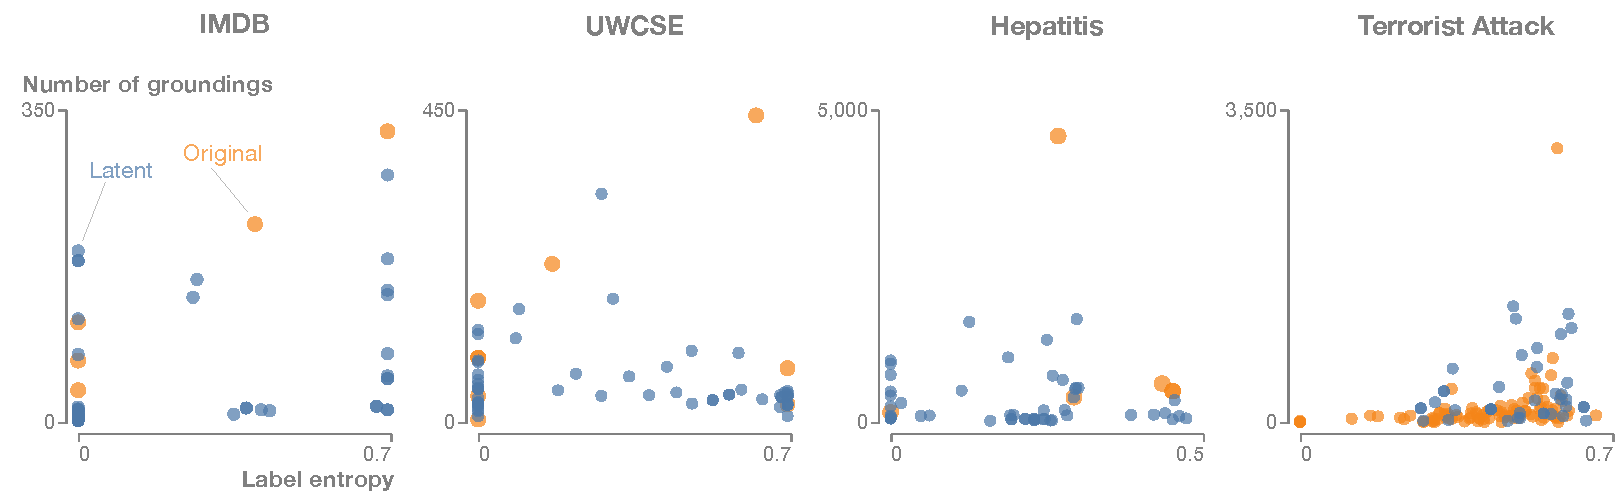
\includegraphics[width=1\textwidth]{combined}
    \caption[Contrasting the label entropy and sparsity in latent representation created by \gls{curled}]{Contrasting the label entropy of predicates and the number of true groundings reveals that the many latent predicates with the low label entropy have similar number of groundings as the predicates of the original data representation. This means that the trivial case, in which a large number of low-entropy predicates is obtained due to many predicates that have just a few true groundings, is not explanation for the experimental results. Instead, the latent representation, when beneficial, successfully identifies local regions in the instance space that match well with the provided labels. The exception to this is again the TerroristAttack dataset.}
    \label{fig:EntropyVsSparsity}
\end{figure}




\textbf{Connecting label entropy and sparsity.}
A potential explanation of the above discussed results might be that many latent features capture a very small number of instances (e.g., 1 or 2) which would lead to a large number of features with low label entropy.
Such features would largely be useless as they make generalisation very difficult.
To verify that this is not the case, Figure~\ref{fig:EntropyVsSparsity} plots the label entropy versus the number of groundings of a predicate.
If latent features of low label entropy would indeed capture only a small number of instances, many points would be condensed in the bottom left corner of the plot.
However, that is not the case -- many latent predicates with low label entropy actually have a number of groundings comparable to the predicates in the original representation.
The exception to this is again the TerroristAttacks dataset.

These results jointly point to the following conclusion: \textit{latent features successfully identify local regions in the instance space that match well with the provided labels}.
As a consequence, these local regions are easier to capture and represent.









\textbf{Redundancy.}
Figure~\ref{fig:Redundancy} summarises the influence of $\alpha$ on the accuracy and the number of latent features.
The figure shows relative reduction in the number of features (equal to the number of predicates), the number of facts and the accuracy with  respect to the latent representation obtained without rejecting the overlapping clusterings.
These results show that the performance of the classifier is not affected by removing features based on the overlap of clusterings they define.
The performance of TILDE remains approximately the same, whereas the number of latent features is reduced by 20 to 30 \%.
As the number of features is directly related to the size of the search space of relational model (and thus the complexity of learning), this is an encouraging result indicating that the size of the search space can be naively reduced without sacrificing the performance.








\begin{figure}[t]
	\centering
	\medskip
    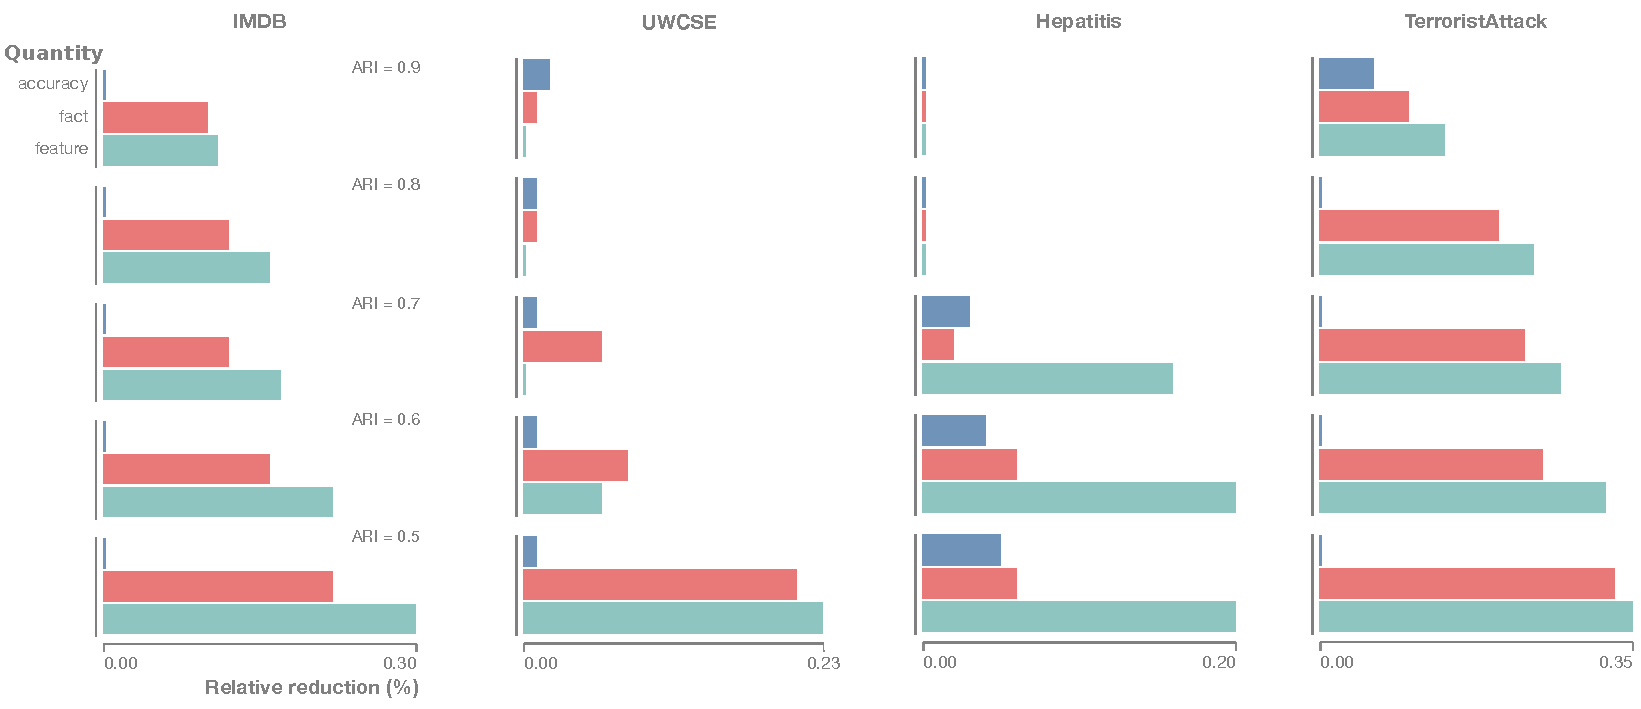
\includegraphics[width=1\textwidth]{redundancy_combined}
    \caption[Redundancy in latent representations created by \gls{curled}]{The performance in terms of the accuracy is barely effected by removing overlapping clusterings, while the number of predicates and facts can be reduced up to 30\%. The only noticeable reduction in performance happen on the Hepatitis dataset, but only for approximately 5\%.   }
    \label{fig:Redundancy}
\end{figure}








\section{On embeddings as an alternative paradigm for relational learning}






\gls{srl} and \gls{kge} methods have largely been developed in isolation and little understanding is currently available on the relative advantages of the respective approaches.
The major strength of \gls{kge}s is their scalability -- they easily operate on knowledge graphs with millions of facts and thousands of relations and the similarity of symbols emerging from the Euclidean space.
As they essentially \textit{vectorize} the data, the scalability of gls{kge}s benefits from very fast computational frameworks leveraging the strengths on GPUs.
Symbolic \gls{srl} methods, on the other hand, are capable of capturing very complex relational patterns, are interpretable and flexible reasoning systems -- once the model of the domain is obtained, a user can pose any query w.r.t. the model and does not have to commit to a predefined target.



The major weakness of \gls{kge}s is that vectorisation of complex relational data is necessarily an \textit{approximation} of it, not the exact re-representation.
We currently lack any measure of the quality of such mapping.
Furthermore, \gls{kge}s are black-box and uninterpretable, limited reasoning capabilities focused on local information, and have a difficult time handling unseen instances.
The weakness of the symbolic \gls{srl} methods is that both inference and learning with such methods is highly complex, limiting its applicability, as well as lack of ways to represent similarity between symbols.



The two respective branches also focus on different tasks.
\gls{kge} methods typically focus on knowledge graph completion which requires very simple forms of relational reasoning. The evaluation metrics are often measuring the quality of rankings generated by the respective scoring functions.
Symbolic \gls{srl} methods typically focus on learning from small relational data, employing more complex forms of logical reasoning.






This work contributes towards a better understanding of the relative strengths and weaknesses of the aforementioned paradigms.
We perform a systematic comparison of \gls{kge}s and symbolic \gls{srl} approaches on various standard relational classification, as well as the knowledge base completion tasks.
Standard relational classification datasets offer a variety of tasks requiring various levels of reasoning complexity, while standard KBC datasets offer insights on real-life large knowledge graphs.
We include both quantitative, in terms of performance, and qualitative analysis, in terms of extracted patterns of reasoning, in order to gain more insights into the suitability of these different methods.









\subsection{Comparing symbolic and distributional methods}


As stated before, the current understanding of the relative strengths and weaknesses of \gls{kge}s and symbolic \gls{srl} methods in very limited.
Several works, however, do offer interesting insights.
Nickel et al. (\cite{NickleNIPS2014}) and Toutanova and Chen (\cite{toutanova2015observed}) show that including both latent features from \gls{kge}s and the observable features, in form of random walks over knowledge graphs, in a join model can greatly increase the performance and reduce the learning complexity.
Pujara et al. (\cite{pujara:emnlp17}) show that \gls{kge}s have difficulties handling data with high degree of sparsity and noise -- which is the case with every automatically created knowledge graph.
Grefenstette (\cite{GrefenstetteTFDS}) introduces a formula framework for simulating logical reasoning through tensor calculation, which can be seen as a form of embeddings that does not require learning.


The work most related to ours is that of Toutanova and Chen (\cite{toutanova2015observed}) and Vig et al. (\cite{VigILP2017}).
Toutanova and Chen compare \gls{kge}s with a simple method that takes the types of incoming edges in a knowledge graph as features (termed observable patterns) and show that such simple observable patterns outperform \gls{kge}s on some datasets.
However, they offer no greater insight in possible reasons.
Vig et al.  compare symbolic \gls{srl} methods with embeddings obtained by the Siamese neural network~\cite{Bromley:1993:SVU:2987189.2987282}, and focus on analysing the impact of the available \textit{background knowledge} on the performance.
Their results indicate that \gls{kge}s might be beneficial when the background knowledge about the task at hand is limited but is such knowledge is available then the symbolic methods are preferable.
Our work presented in this paper differs in a way that it goes beyond quantitative analysis and includes substantial qualitative analysis with respect to the complexity of reasoning needed to address the task.



\subsection{Aims, Materials and Methods}

The main goal of this study is to identify the strengths and weaknesses of  \gls{kge} and symbolic \gls{srl} approaches to learning and reasoning with relational data.
Concretely, we focus on the following question:

\begin{displayquote}
\textit{Are \gls{kge}s a viable alternative to symbolic methods for relational classification?}
\end{displayquote}

%\begin{itemize}
%	\setlength{\itemindent}{1em}
%	\item[\textbf{Q1}] \textit{Are KGEs a viable alternative to logic-based methods for relational classification?}
%	\item[\textbf{Q2}] \textit{Are KGEs a viable alternative for relational clustering methods?}
%\end{itemize}

\noindent More specifically, we focus on the following task

\begin{displayquote}
\textit{Given a set of \textbf{target instances} (entities in a knowledge base), learn a model that predicts the value of the labels associated with those instances. We consider fully relational models learning the logical theory for predicting the labels, and a feature based models learning from the vector representation of target instances.}
\end{displayquote}


Our focus is exclusively on the classification tasks as they give us a well-defined and clear performance measure, in contrast to the clustering task which is ill-defined ~\cite{Estivill-Castro:2002}.






\gls{kge} methods are usually trained to assign a high score to all facts in a knowledge base, not to specific \textit{target} facts.
To make sure this training criterion does not put \gls{kge}s at a disadvantage, once the embeddings are obtained, we use them as the input data for a classifier learning the predictive model for the pre-specified target.



As \gls{kge} methods are focused on the knowledge graph completion task, they assume that all instances are given at once and focus on filling in the missing links in data.
Therefore, they have difficulties with unseen instances.
We do not address this issue here, but simply learn the representation of both training and test data at the same time (with labels excluded).
It is, however, worth noting that \gls{kge} methods have a certain advantage due to this.




\subsubsection{Materials}



\paragraph{Relational classification dataset}
We take standard relational learning datasets and use the available labels as ground truth for both classification and clustering.
The IMDB dataset is a snapshot of the Internet Movie Database, describing a set of movies with their actors and directors.
The task is to distinguish between actors and directors.
The UWCSE dataset describes the employees of the University of Washington, their roles, publications, and courses.
The task is to distinguish between students and professors.
The Mutagenesis dataset consists of a set of molecules and their structures, with the goal of predicting whether a compound is mutagenic or not.
The Carcinogenesis data is a similar dataset, but focuses on a different compound property.
The Yeast dataset describes a data about regulatory paths in the genome of yeast, and the target is to predict active paths.
The WebKB dataset describes web pages of four US universities and their corresponding link structure.
The pages are classified into seven groups according to their roles such as personal, departmental or project page.
The Terrorists dataset contains a network of terrorist attacks, each assigned to of the 6 types of attacks.
Finally, the Hepatitis dataset describes a set of patients with a diagnosis of Hepatitis B and C.
We intentionally focus on standard relational learning datasets because they typically expose a more variety of reasoning: required reasoning ranges from attribute-only reasoning to multi-hop reasoning.
Some of the properties are listed in Table~\ref{tab:properties}.
For each property, we differentiate between target instances -- instances which contain labels, and the rest.
This gives us a better opportunity to detect the conditions under which either of the respective approaches is preferable.
In contrast, standard KB completion datasets are often very simple and  only simple path-type rules are required to achieve a reasonable performance.
Therefore, the disadvantage of standard relational methods is that they might very inefficient because of the dataset size.
Additionally, if the provided data does not contain useful features, KGE methods might still be able to extract certain useful patterns through the latent features.



\begin{table}[t]
	\centering

	\caption[Properties of the relational classification datasets]{Dataset properties summarise the number of target and all instances, the number of attributes, and the number of relation types.}
		\begin{tabular}{@{}lcccccc@{}}
			\toprule
			\textbf{Dataset} 	& \multicolumn{2}{c}{\textbf{Instances}} 		& \multicolumn{2}{c}{\textbf{Attributes}}	& \multicolumn{2}{c}{\textbf{Relations}} \\
								\cmidrule(rl){2-3} \cmidrule(lr){4-5} \cmidrule(l){6-7}
								& Target 				& Total					&   Target				& Total				& Target		& Total						\\
			\midrule
			Hepa				& 500					& 5919					& 2						& 12				& 3				& 3						\\
			Muta				& 230					& 6124					& 3						& 7					& 3				& 7						\\
			Terror				& 1293					& 1293					& 104					& 104				& 2				& 2						\\
			WebKB				& 920					& 3880					& 763					& 1207				& 4				& 5						\\
			Carc				& 1700					& 45940					& 0						& 71				& 28			& 28 \\
			Yeast				& 13750					& 13750					& 1836					& 1836				& 1				& 1 \\
			UWCSE				& 2824					& 3714					& 0						& 23				& 1				& 5 \\
			\bottomrule
		\end{tabular}
	\label{tab:properties}
\end{table}


\paragraph{Knowledge base completion datasets}
Our experiments include standard KBC datasets, FB15k-237 and WN18-RR.
FB15k-237~\cite{toutanova2015observed} is a subset of Freebase which contains approximately 15000 entities and 237 relations; this is an improved version of the predecessor FB15k, but with inverse relations removed, which gave overly optimistic performance \cite{toutanova2015observed}.
WN18-RR~\cite{dettmers2018conve} is a subset of the WordNet knowledge graph, consisting of approximately 50 000 entities and 11 relations.
It is an improved version of the WN18 dataset, which had the same problem as FB15k.




\paragraph{Knowledge graph embeddings}
Due to the sheer magnitude of the existing \gls{kge} methods \cite{EmbeddingsOverview}, including a large sample in the comparison would be infeasible.
Moreover, it is not clear whether a big difference in performance is expected~\cite{DBLP:conf/rep4nlp/KadlecBK17}.
Therefore, we focus on the two prototypical and, arguably, most used approaches -- TransE and DistMult, as well as the state-of-the-art approach of ComplEx \cite{trouillon2016complex}.
It is important to note that ComplEx produces embeddings in the \textit{complex Euclidean space} and that each entity is associated with two embeddings - \textit{real} and \textit{imaginary} one.
In order to create a single embedding out of these two, we consider three version of ComplEx embeddings: (1) taking an average of two embeddings, (2) their sum, and (3) concatenation of two embeddings.




\paragraph{Classifiers}
\newglossaryentry{kfoil}{name={kFOIL},description={kFOIL}}
When using machine learning algorithms for prediction, it is important to consider the bias an algorithm introduces.
To better understand how the difference in performance between \gls{kge}s and symbolic \gls{srl} methods is influenced by the bias of the particular machine learning algorithm, we experiment with three different ML families -- decision trees (DT), support vector machines (SVM) and $k$ nearest neighbours (kNN), and their relational counterparts -- relational decision tree TILDE~\cite{Blockeel1998285}, relational kernel machines \gls{kfoil}~\cite{Landwehr:2006:KLS:1597538.1597601} and kNN with a relational similarity measure of ReCeNT~\cite{Dumancic2017a}.










\subsubsection{Methods}


\paragraph{Relational classification}
We perform standard nested cross-validation.
For each split, the training data is used to learn the models and tune their parameters (using an inner cross-validation loop) and the unseen fold is used for testing.
We report the relative performance of KGEs to the relational baseline in terms of the difference in the accuracies, $acc_{KGE} - acc_{relational~ baseline}$, averaged over individual splits.
The labels were excluded from the data when learning the \gls{kge}s and considered only during the training of the classifier.


The embeddings of each relational data were obtained before learning a classifier.
The dimensions of the embeddings were varied in $\{10, 20, 30, 50, 80, 100\}$; we include smaller dimensions because standard relational datasets tend to have a much smaller number of entities than the KBC datasets (see Table \ref{tab:properties}).
All embeddings were trained to 100 epochs and saved in steps of 20.
We do not use the validation set and metrics such as mean reciprocal rank to select the best hyper-parameters for the embeddings, as they may not be perfectly correlated with the predictive accuracy; instead, we treat the dimension and the number of epochs for training as additional parameters while training the classifiers as part of the inner cross-validation loop.


\paragraph{Knowledge base completion}
For the experiments with the knowledge base completion datasets, we do not re-train the KGEs but report the results from \cite{dettmers2018conve} which are considered to be state-of-the-art.
These experiments include several methods: DistMult~\cite{YangYHGD14a}, ComplEx~\cite{trouillon2016complex}, R-CGN~\cite{Schlichtkrull2017ModelingRD} and ConvE~\cite{dettmers2018conve}.
Relational decision tree TILDE is used as a relational baseline due to its simplicity and speed.
One model is trained for each relation, and the mean and weighted (by the number of examples in the relation) accuracy is reported.
The training procedure is the same as for the experiments regarding the relational classification datasets, with an exception that only one (pre-defined) test split is used.
KGEs are usually evaluated by how well they rank the correct answers to a triple in which either the subject or objects are left out (i.e, $<\mathbf{s},\mathbf{r},\mathbf{?}>$ or $<\mathbf{?},\mathbf{r},\mathbf{?}>$), and the metrics used are ranking measure such as \textit{mean reciprocal rank} and \textit{hits @ K} (\textit{is the correct answer among the top K ranked answers}) \cite{Bordes:2013:TEM}.
Such rankings are difficult to obtain with the ILP methods, which makes the comparison somewhat difficult.
As Hits@1 directly correspond to the accuracy, and we use this as a primary mean of the comparison.







\subsection{Comparative results}

\subsubsection{Relational classification}


\begin{figure}[!ht]
	\centering
	\begin{subfigure}{0.98\linewidth}
		\centering
		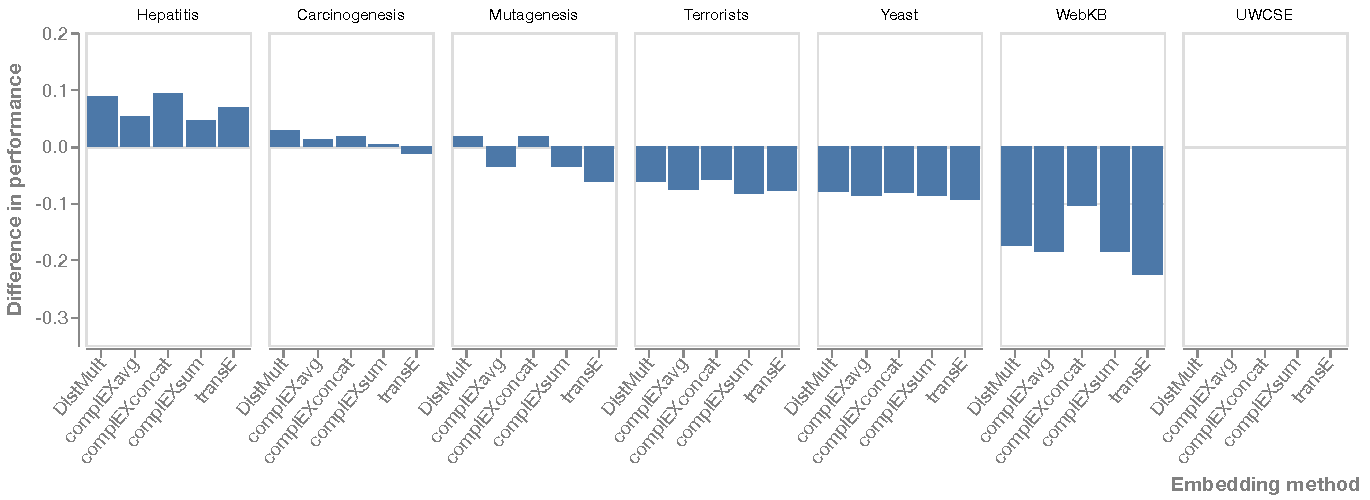
\includegraphics[width=.95\linewidth]{decisiontrees}
		\caption{Performance with decision trees\label{fig:dtres}}
	\end{subfigure}

	\begin{subfigure}{0.98\linewidth}
		\centering
		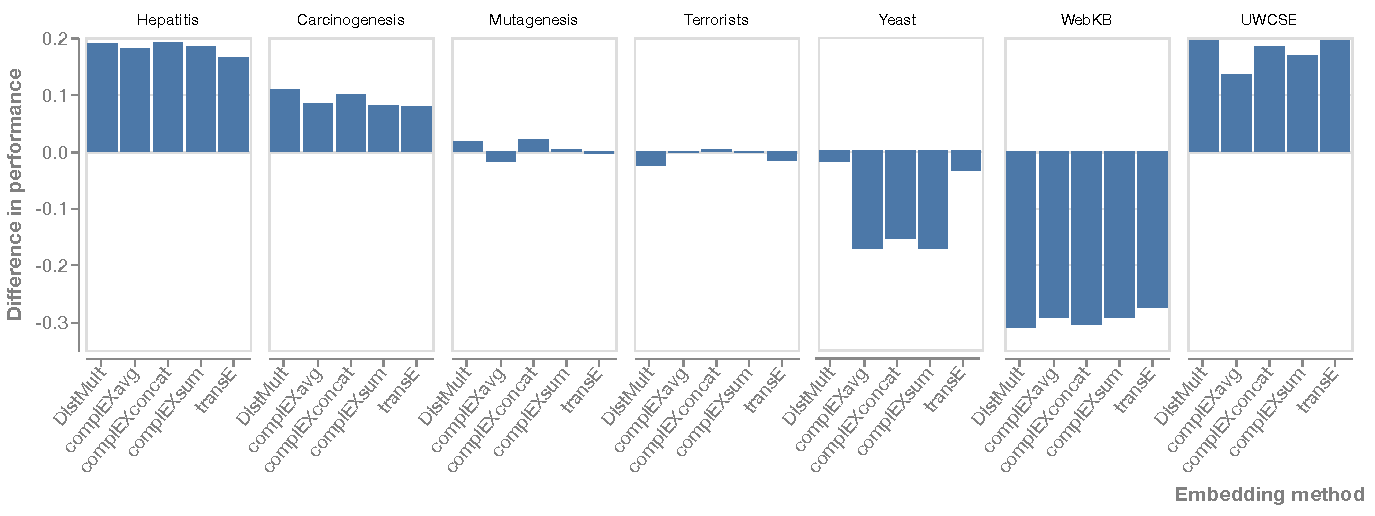
\includegraphics[width=.95\linewidth]{svms}

		\caption{Performance with svms\label{fig:svms}}
	\end{subfigure}

	\begin{subfigure}{0.98\linewidth}
		\centering
		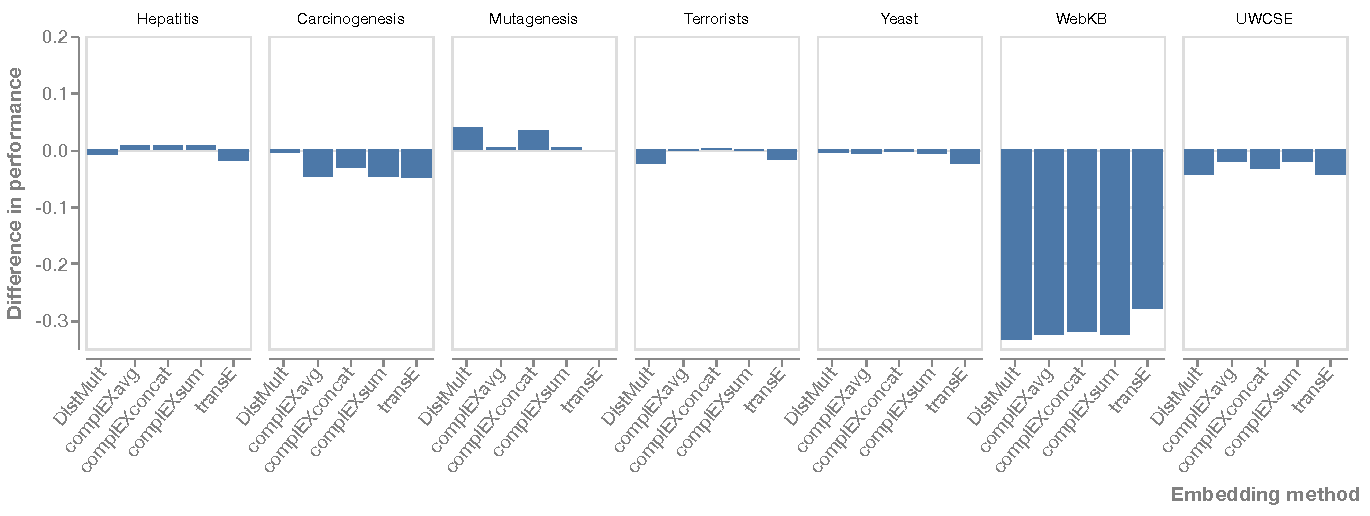
\includegraphics[width=.95\linewidth]{knns}

		\caption{Performance with kNNs\label{fig:knns}}
	\end{subfigure}

	\caption{Performance with different classifiers on the relational classification problems}
\end{figure}








The experiments with (relational) decision trees (Figure \ref{fig:dtres}) indicate that the decision tree trained on the embeddings features outperform TILDE only on two datasets-- Hepatitis and Carcinogenesis, while performance is equal on the UWCSE dataset.
The results also indicate that the performance of various KGE models is relatively similar, but \textit{DistMult} and \textit{ComplEXconcat} seem to have a slight edge.



What is most interesting in these results is not the difference in the performance itself, but \textit{whether we could explain what gives \gls{kge} methods (dis)advantage on certain datasets?}
In order to do so, we analyse the results with respect to the semantics of the predicates used in the extracted rules, which yields further interesting results.
More precisely, we differentiate between \textit{attribute predicates} that associate a specific value of an attribute with an instance, and \textit{relation predicates} that connect two instances.
We further distinguish between \textit{target} instances having an associated label, and \textit{neighbourhood} instances that provide additional data.
Table~\ref{tab:ruleproperties} summarises the rules extracted by TILDE w.r.t. the above-discussed interpretation.



\begin{table}[h!]
	\centering

	\caption[Properties of the extracted rules]{Properties of extracted rules are summarised as a proportion of relation and attribute predicates they contain. \textit{Rule properties} section describes the proportion of rules that contain  \textit{relation} predicates only, \textit{attribute} predicates only and the mix of both, for each dataset. \textit{Dataset properties} section shows the proportion of possible attribute and relation predicates that are used in the extracted rules. For example, the rules on the Hepatitis dataset use 100 \% of the possible attribute predicates, and 66 \% of relation predicates. \textit{Neighbourhood} refers to the proportion of attribute and relation predicates of the non-target instances for which a direct link with target instances exists. }
	\resizebox{.95\linewidth}{!}{
		\begin{tabular}{@{}lccccccc@{}}
			\toprule
			\textbf{Dataset}		& \textbf{Model} 	& \multicolumn{3}{c}{\textbf{Rule properties}} 	& \multicolumn{3}{c}{\textbf{Dataset properties}} \\
			\cmidrule(lr){3-5} \cmidrule(l){6-8}
								& \textbf{complexity}		& Relations   		& Attributes 	& Mix		& Attributes        & Relations	& Neighbourhood	     \\
								\midrule
			Hepatitis   		& 15					  		& 10 \%				& 38 \%			& 52 \%		& 100 \%					&  66 \%				& 70 \%				\\
			Carcinogenesis		& 24							& 0 \%				& 0 \%			& 100\%		& 	--	 			& 100 \% & 72 \% \\
			UWCSE				& 35.5						& 0 \%				& 2 \%			& 98 \%		&	75 \%			&	80 \%		& 0 \% \\
			Terrorists			& 17.65						& 0	\%				& 95 \%			& 5 \%		& 35 \%				& 100 \%		& 0 \%			\\
			Mutagenesis			& 9.4						& 0 \%				& 100 \%		& 0 \%		& 100 \%					& 0 \%	& 0 \%				\\
			WebKB				& 38							& 5 \%				& 76 \%			& 19 \%		& 4 \%				& 50 \%		& 1 \%		\\

			Yeast 				& 188.4						& 0 \%				& 8 \%			& 92 \%		& 78 \%				&	100 \%		& -- \\
			\bottomrule
		\end{tabular}
	}
	\label{tab:ruleproperties}
\end{table}




The results indicate an interesting connection between the performance and the amount of data information that is found predictive: the properties of TILDE rules extracted for the Hepatitis and Carcinogenesis datasets reveal that the majority of provided information, both attributes and relations, are found predictive.
For instance, on the Hepatitis dataset,  the induced rules incorporate 100 \% of the target attributes and 66 \% of relations involving target instances, as well as 70 \% of the predicates related to the neighbouring instances.
Similar numbers hold for the Carcinogenesis data.



The remaining datasets are different in that regard -- only a fraction of information is found predictive.
On the Mutagenesis dataset\footnote{we use the version of the dataset without any rings structures and additional background knowledge which is difficult to incorporate in \gls{kge} methods}, even though all the attributes of molecules are found predictive, none of the relations were found predictive and thus none of the information about atoms they contain.
Thus, only a fraction of available information is used.
On the WebKB dataset, only 4 \% of the attributes have been found predictive, as well as 50 \% of relations.



The results and the analysis of the rules suggest that \gls{kge} have an edge over the \gls{srl} methods when \textit{most of the information in the neighbourhood of instances is relevant}.
An explanation for such a big difference in performance might be that SRL methods have to select few predictive rules while learning theories, and thus can discard irrelevant information.
In contrast, the learning principle of KGEs is designed to take all of the information into account, which seems to make them underperform.




A similar trend is also evident when the (relational) SVM is used as a classifier.
However, \gls{kge}-based methods achieve better relative performance on the Hepatitis, Carcinogenesis and UWCSE dataset, while the difference in performance is much less pronounced on the Mutagenesis and Terrorists datasets.
It is interesting to note that symbolic and \gls{kge}-based methods do not benefit equally by using the more powerful learner.
We attribute this to the fact that kFOIL essentially creates a \textit{binary embedding} -- it identifies a set of useful relational features (similar to random walks), followed by learning a kernel SVM on such binary data.
Therefore,  it is closer to the \gls{kge}-based methods than the fully relational once, and it is likely that it loses some of the semantics of relational data by binarising it.



The pattern, however, disappears with the kNN classifier.
Whereas previously \gls{kge}-based methods substantially outperformed symbolic methods on the Hepatitis, Carcinogenesis and UWCSE datasets, relational versions of kNN perform equally well on the Hepatitis dataset and outperform \gls{kge}-based methods on the Carcinogenesis and UWCSE datasets.
\gls{kge}-based methods seem to gain the advantage on the Mutagenesis dataset, but the remaining datasets prefer symbolic approaches.
However, a general trend is that the differences in performances are much less pronounced compared to the results with decision trees and SVMs, except on the WebKB.
We suspect that the reason for this is that similarity is difficult to measure with relational data, despite a considerable body of work addressing the problem \cite{Dumancic2017a}, and \gls{kge}s might be a viable alternative.



To validate our conclusion, we design a control experiment focusing on the WebKB dataset where the difference in performance is the largest.
We created the second version of the dataset that contains only the information, both relations and attributes, deemed useful by the symbolic \gls{srl} methods.
More precisely, in the case of decision trees, we take the information deemed useful by decision trees, while in the case of SVM we take the information found useful by kFOIL.
For the case of kNN, it is not easy to identify the exact information that makes the most influence on the relational similarity measure; therefore, we use the information identified by TILDE and kFOIL.
If our observation is correct and not the result of randomness, the performance of \gls{kge}s should improve on this filtered version of the dataset.
The results (Figure \ref{fig:filter_results}) do confirm so: the difference in performance of \gls{kge}s and symbolic \gls{srl} methods reduces in the cases of decision trees (Figure \ref{fig:dt_difference}) and SVMs (Figure \ref{fig:svm_difference}), especially when decision trees are used.
Interestingly, TransE and DistMult seem to benefit from that more than ComplEx.
The differences in performance between \gls{kge}s and symbolic \gls{srl} methods do not disappear completely -- we attribute this to the sparsity of the filtered graph, as it is known that the quality of the embeddings relies on the level sparsity of the knowledge graph~\cite{pujara:emnlp17}.
Moreover, filtering the data might have filtered out some of the useful information that coincidentally correlates well with information deemed useful by the symbolic learner.
Thus, the inclusion of such information might be beneficial to \gls{kge}s, but we do not have a way to detect it easily.
Moreover, we have noticed that there is a relatively small overlap between information found predictive by TILDE and kFOIL, indicating that the bias of the learning algorithm plays an important role in detecting which parts of the available information is predictive.
The kNN results again diverge from this trend, and the results suggest that KGE-based methods perform worse than with the unfiltered dataset.
The likely reason for that is that the filtered information matches the bias of decision trees and SVMs, but not the kNNs similarity measure, and further confirms that measuring the similarity in relational data is a difficult problem.



\begin{figure}
	\centering
	\begin{subfigure}{0.32\linewidth}
		\centering
		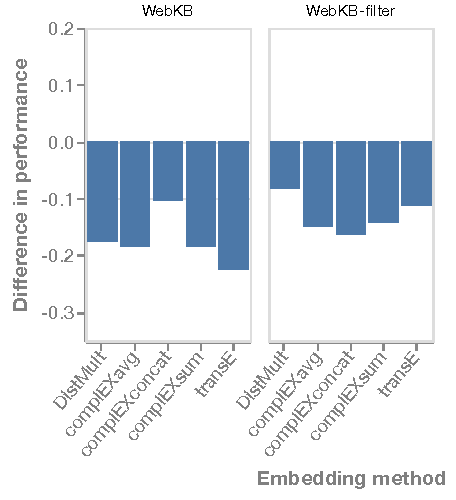
\includegraphics[width=.85\linewidth]{dt_filter}
		\caption{Decision trees \label{fig:dt_difference}}
	\end{subfigure}
	\begin{subfigure}{0.32\linewidth}
		\centering
		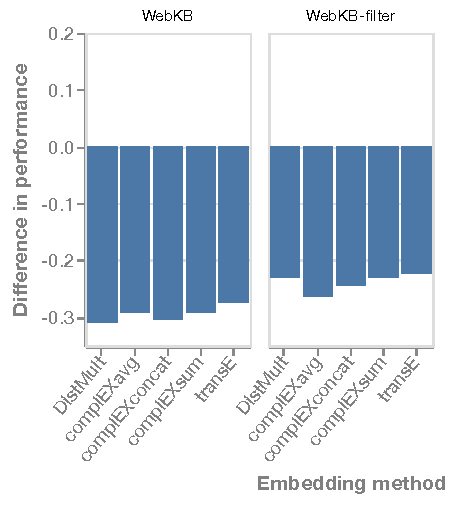
\includegraphics[width=.85\linewidth]{svm_difference}
		\caption{SVM \label{fig:svm_difference}}
	\end{subfigure}
	\begin{subfigure}{0.32\linewidth}
		\centering
		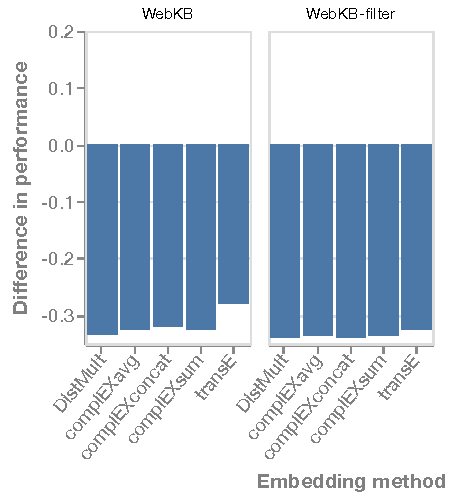
\includegraphics[width=.85\linewidth]{knn_difference}
		\caption{kNN \label{fig:knn_difference}}
	\end{subfigure}
	\caption[Control experiment - results on the filtered version of the WebKB dataset]{Results on the filtered version of the WebKB dataset show the improvement in the performance of \gls{kge}-based methods in combination with decision trees and SVMs, but not when kNN is used.}
	\label{fig:filter_results}
\end{figure}








\subsubsection{Knowledge base completion}


\begin{table*}[h]
	\centering
	\caption{Performance on the knowledge base completion tasks}
	\label{tab:kbcres}
	\resizebox{\linewidth}{!}{%
		\begin{tabular}{@{}lrrrrrr@{}}
		\toprule
						& \multicolumn{3}{c}{\textbf{FB15-237}} & \multicolumn{3}{c}{\textbf{WN18-RR}} \\
			\cmidrule(lr){2-4} \cmidrule{5-7}

						& Mean accuracy & Weighted accuracy & Mean complexity 	& Mean accuracy & Weighted accuracy & Mean complexity \\
			\midrule

		\textbf{TILDE} 	& .95			& .98				& 10.15			  	& .90			& .83				& 231 \\
		\midrule
						& Hits@1			& Hits@3 			& Hits@10			& Hits@1			& Hits@3 			& Hits@10 \\
						\cmidrule(lr){2-4} \cmidrule{5-7}
		\textbf{ConvE}	&	.327			&	.356				&	.501				& .40				&	.44				&	.52		\\
		\textbf{Complex}&	.158			&	.275				&	.428				& .41				&	.46				&	.51		\\
		\textbf{DistMult}&	.155			&	.263				&	.419				&	.39				&	.44				&	.49		\\
		\textbf{R-GCN}	&	.153			&	.258				&	.417				&	--				&		--			&		--	\\
		\bottomrule


		\end{tabular}
	}
\end{table*}


The results on the KBC datasets (Table \ref{tab:kbcres}) indicate that the symbolic SRL methods perform rather well on these datasets.
On the FB15k-237 dataset, TILDE achieves the mean accuracy of 95\% and the weighted mean accuracy of 98\% while inducing relatively simple model having on average 10.15 nodes in the tree.
The WN18-RR dataset is rather different than the FB15k-237: TILDE achieves the mean accuracy of 90\% but the weighted mean accuracy of 83\% which means that the relations with a higher number of test examples are predicate less accurately.
The results show that this dataset is much more complex than the FB15k-237 as it requires rather long chains of reasoning, indicated by large TILDE trees having on average 231 nodes.


The performance of \gls{kge} methods lags behind.
On the FB15k-237 dataset, the best-performing methods in ConvE with Hits@1 of .327 and Hits@10 at .501.
On the WN18-RR dataset, ConvE also performs the best with Hits@1 of 0.40 and Hits@10 of 0.52.
These results are consistent with the conclusion from the experiments on relational classification: the size of TILDE trees indicate the relevant information requires several \textit{hops} in a knowledge graph and it is not in the intermediate neighbourhood of entities.





\subsection{Key messages}


Many problems nowadays are naturally expressed in form of relational and graph structures data.
This includes social and protein interaction networks, biological data, knowledge graphs and many more.
Two main machine learning paradigms for analysing such data, knowledge graphs embeddings and  symbolic statistical relational learning, have mostly been studied in isolation so far.
This work is the first, to the best of our knowledge, that systematically compares these two paradigms on the standard tasks from both domains -- relational classification and knowledge base completion.
Our results point to the following conclusion:
\begin{itemize}
	\item \textbf{\gls{kge}s seems to be suitable for curated data.}  KGEs seem to be at a disadvantage when only a small fraction of available information is useful for the given prediction task. Symbolic SRL methods do not have that issue as they can cherry pick useful information during the learning phase. This conclusion was further confirmed by the control experiment in which the uninformative data (as found by the symbolic methods) was removed from the dataset -- the difference in performance between KGEs and symbolic methods has decreased.
	\item  \textbf{Symbolic methods outperform KGEs on knowledge base completion tasks.} We have noticed a large gap in the performance between symbolic and KGE methods when compared on the standard KBC datasets: whereas symbolic methods achieve accuracy $> 90$\%, KGE methods struggle and achieve the accuracy $\approx 50$\%. This suggests that the KGEs, at least in the current state, are more suitable for the interactive inspections of large knowledge graphs than for the automatic reasoning.
	\item \textbf{KGEs might be a good way to measure the similarity in relational data.} On most datasets, KGE and symbolic methods had almost identical performance when learning based on similarities was employed. This suggests that KGE-based similarity is competitive with the large body of works on this problem.
\end{itemize}

This work is not meant as a criticism of any of the considered approaches but hopes to identify \textit{useful bits} of individual approaches that might be worth integrating.
We hope this work inspires new research directions focused on combining the strengths of both approaches as both communities has already started to explore \cite{DBLP:conf/uai/MinerviniDRR17,demeester2016lifted,Schlichtkrull2017ModelingRD}.





\begin{tcolorbox}[enhanced,attach boxed title to top center={yshift=-3mm,yshifttext=-1mm}, colback=blue!5!white, colframe=blue!75!black, colbacktitle=white, coltitle=red!25!black,
title=Intermezzo: DeepProbLog,fonttitle=\bfseries, boxed title style={size=small,colframe=blue!75!black} ]

	Symbolic methods for representation learning with relational data are in the focus of this thesis.
	The experimental analysis presented in this chapter clearly shows that both research directions have strengths and weaknesses.
	Moreover, a general consensus is that deep learning excels at perception tasks such as object recognition in images, whereas symbolic approaches excel at reasoning.
	Therefore, investigating the closer integration of symbolic and deep approaches deserves attention. \\


	Manhaeve et al.~\cite{DBLP:journals/corr/abs-1805-10872} introduce \texttt{DeepProbLog} -- an extension of \texttt{Problog} with the support for \textit{neural predicates}.
	\texttt{DeepProbLog} starts from the perspective that explicitly specifying the probabilities of all probabilistic facts in a domain might be difficult for certain tasks, if not impossible.
	For instance, various perception tasks require large image datasets for learning a well-performing model; manually annotating the probabilities of certain objects being detected in all images is impossible.
	the core idea of \texttt{DeepProbLog} is to introduce a new construct, the \textit{neural predicate}, that allows a user to provide a \textit{neural model} that can estimate the probabilities of grounded atoms being \texttt{true} given the arguments of the atom.
	The neural model does not have to be trained beforehand, but can be learned from scratch given the examples of a target task. \\


	Formally, \texttt{DeepProbLog} extends the concept of \textit{annotated disjunction}.
	Annotated disjunction is an expression of the form
	\begin{center}
		\texttt{p$_1${::}h$_1$; \ldots; p$_n${::}h$_n$ {:-} b$_1$,\ldots,b$_m$.}
	\end{center}
	where \texttt{p$_i$} are probabilities to that $\sum_ip_i=1$, and \texttt{h$_i$} and \texttt{b$_j$} are atoms.
	The meaning of the annotated disjunction is that whenever all \texttt{b$_i$} are \texttt{true}, \texttt{h$_j$} will be true with probability \texttt{p$_j$} with all other \texttt{h$_{i \neq j}$} being \texttt{false}.
	\texttt{DeepProbLog} introduces a \textit{neural} annotated disjunction of the form
	\begin{center}
			$nn(m_q,\vec{t}, \vec{u}) :: q(\vec{t},u_1); \ldots; nn(m_q,\vec{t}, \vec{u}) :: q(\vec{t},u_n) $ \texttt{{:-} b$_1$,\ldots,b$_m$.}
	\end{center}
	where $nn$ is a neural model, $\vec{t}$ is a vector of ground terms representing the inputs of a neural model for predicate $q$, $u_i$ are possible output values of the neural model.
	$m_q$ is the identifier of a neural model that specifies a probability distribution over output values $\vec{u}$ given the output $\vec{t}$
\end{tcolorbox}


\section{Conclusion}


This chapter digs deeper into the properties of relational latent representations.
It first inspects latent representations created by \gls{curled} showing that such latent representations improve the performance of relational learners by capturing small local regions in data that match well with the labels.
It demonstrates that by showing that the predicates in the latent representation are sparser but with the reduced label entropy.
The analysis also shows that the \gls{curled}-created latent features tend to be redundant and shows that the number of latent features can be reduced without sacrificing the performance.
The chapter then focuses on comparing the \gls{kge} and \gls{ilp} approaches to relational learning on various benchmarks.
This second analysis shows that \gls{kge}s outperform \gls{ilp} methods on relational classification tasks when the data is curated -- the data contains only the relevant information.
In the scenarios when that is not the case, \gls{ilp} have an edge over the \gls{kge} methods.
The analysis also shows that \gls{ilp} methods outperform \gls{kge}s on the standard knowledge base completion tasks, while embeddings seem to be an interesting approach for assessing the similarity of relational objects.



%%%%%%%%%%%%%%%%%%%%%%%%%%%%%%%%%%%%%%%%%%%%%%%%%%
% Keep the following \cleardoublepage at the end of this file,
% otherwise \includeonly includes empty pages.
\cleardoublepage

% vim: tw=70 nocindent expandtab foldmethod=marker foldmarker={{{}{,}{}}}
